% TEXINPUTS=.:$HOME/git/bvtex: latexmk  -pdf <main>.tex
\documentclass[xcolor=dvipsnames]{beamer}

\input{defaults}
\input{beamer/preamble}

\setbeamertemplate{navigation symbols}{}
% \setbeamertemplate{background}[grid][step=1cm]

\usepackage{siunitx}
\usepackage{xmpmulti}
\usepackage[export]{adjustbox}

\usepackage[outline]{contour}
\usepackage{tikz}
\usetikzlibrary{shapes.geometric, arrows}
\usetikzlibrary{positioning}

\definecolor{bvtitlecolor}{rgb}{0.98, 0.92, 0.84}
\definecolor{bvoutline}{rgb}{0.1, 0.1, 0.1}

\renewcommand{\bvtitleauthor}{Brett Viren}
\renewcommand{\bvtit}{LARF}
\renewcommand{\bvtitle}{\LARGE \textbf{LArTPC Detector Response Calculations}\\Using \textbf{B}oundary \textbf{E}lement \textbf{M}ethod}
\renewcommand{\bvevent}{$\mu$Boone Sim\\12 Jul 2016}
\renewcommand{\bvbeamerbackground}{}

\newcommand{\microboone}{MicroBooNE\xspace}


\begin{document}
\input{beamer/title.tex}

\begin{frame}
  \frametitle{Method Overview}
  \href{https://en.wikipedia.org/wiki/Boundary_element_method}{Boundary Element Method} (BEM)
  \begin{enumerate}\footnotesize
  \item Discretize (mesh) boundary electrode surfaces.
  \item Define (Dirichlet) scalar potential on each mesh element (triangle).
  \item Calculate (Neumann) vector normal potential.
  \item Integrate Laplace equation $\nabla^2\phi=0$, evaluate at boundary.
  \item Evaluate solution across a \textbf{grid of points} in the volume.
    \begin{itemize}\scriptsize
    \item[$\rightarrow$] \textbf{electrostatic drift} and \textbf{Shockley-Ramo weighting} potentials.
    \end{itemize}
  \end{enumerate}
  
  Stepping method:
  \begin{itemize}\footnotesize
  \item Instantaneous Shockley-Ramo current in $k^{th}$ wire: \\
    \begin{center}
      $i_k = q \times \mu \times (\vec{E}_{weight,k} \cdot \vec{E}_{drift})$      
    \end{center}
  \item Adaptive Runge-Kutta+Cash/Karp stepping through velocity field:
    \begin{center}
      $\vec{v} = \mu \times \vec{E}_{drift}$      
    \end{center}
    
  \item Raster each linear step to a scale comparable to \textbf{grid points}.
  \item Discretize current ($i_k$) samples to make ``digitized'' waveforms.
  \end{itemize}

\end{frame}

\begin{frame}
  \frametitle{Element Methods: Boundary vs. Finite}
  \begin{columns}
    \begin{column}{0.5\textwidth}
      BEM
      \begin{itemize}\footnotesize
      \item Meshes the surfaces.
      \item Fast for low surface-to-volume.
      \item Performance relies on newish mathematical developments.
      \item Relatively few software implementations.
      \end{itemize}      
    \end{column}
    \begin{column}{0.5\textwidth}
      FEM
      \begin{itemize}\footnotesize
      \item Meshes the volume.
      \item Fast for high surface-to-volume.
      \item Adaptive meshes can improve performance.
      \item Many implementations, heavily used in industry.
      \end{itemize}      
    \end{column}
  \end{columns}

  \vspace{10mm}

  Can also consider a unified/hybrid BEM/FEM calculation.  
  \begin{itemize}
  \item BEM in the volume,
  \item   FEM in near the surface.
  \end{itemize}
\end{frame}

\begin{frame}
  \frametitle{Wire Meshes}

  \footnotesize

  \begin{columns}
    \begin{column}{0.3\textwidth}
      \begin{center}
        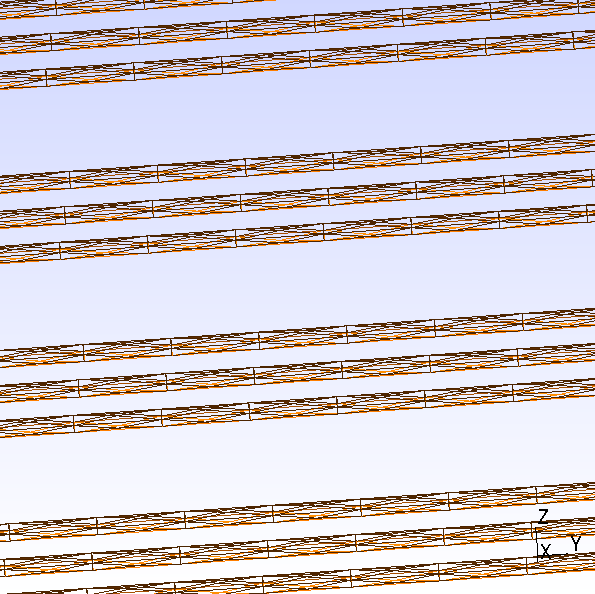
\includegraphics[height=0.4\textheight]{parallel-mesh.png}      
        
        ``Parallel'':\\3mm pitch and gap\\all wires parallel
      \end{center}
    \end{column}
    \begin{column}{0.3\textwidth}
      \begin{center}
        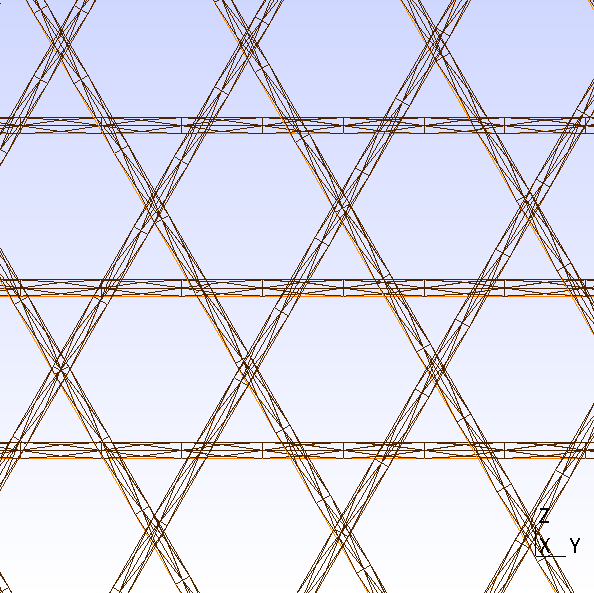
\includegraphics[height=0.4\textheight]{uboone-mesh.png}      

        ``MicroBooNE'':\\3mm pitch and gap\\$60^\circ$ angles for U/V.
      \end{center}
    \end{column}
    \begin{column}{0.3\textwidth}
      \begin{center}
        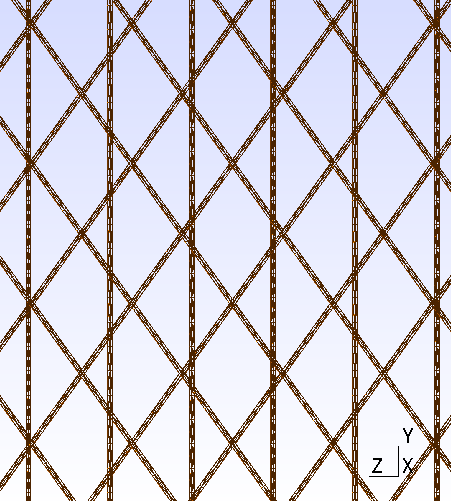
\includegraphics[height=0.4\textheight]{dune-mesh.png}      

        ``DUNE'':\\5mm pitch and gap\\$35.7^\circ$ angles for U/V.
      \end{center}
    \end{column}
  \end{columns}

  \vspace{4mm}

  \begin{itemize}
  \item ``Parallel'' used to reproduce 2D calculations. 
  \item Geometry parameterized to facilitate exploring different configurations.
  \end{itemize}

\end{frame}


\begin{frame}
  \frametitle{MicroBooNE Patch}

  \begin{center}
    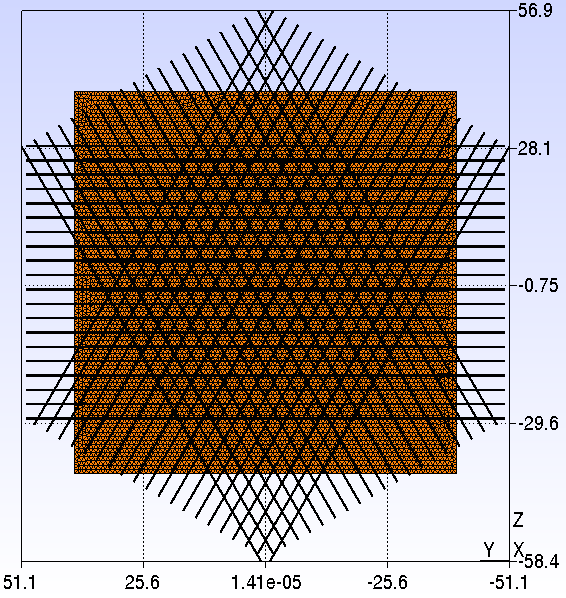
\includegraphics[height=0.7\textheight]{uboone-mesh-with-plate.png}%
    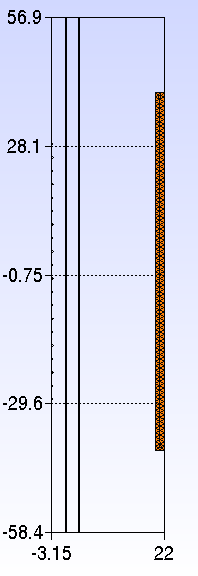
\includegraphics[height=0.7\textheight]{uboone-mesh-with-plate-side.png}      

    \begin{itemize}\footnotesize
    \item ``Cathode'' is close to wires with voltage adjusted to give 500V/cm.
    \item Do calculations near center, far enough away from edge effects.
    \end{itemize}
  \end{center}

\end{frame}


\begin{frame}
  \frametitle{Weighting Potential - 2D vs ``2D''}

  \vspace{-5mm}

  \begin{columns}
    \begin{column}{0.5\textwidth}
      \begin{center}
        \includegraphics[height=0.65\textheight,page=5,angle=-90,clip,trim=0 0 0 5mm]{GarfieldSimulation-BoYu.pdf}

        \scriptsize Garfield 2D calculation from Bo
      \end{center}
    \end{column}
    \begin{column}{0.5\textwidth}
      \begin{center}
        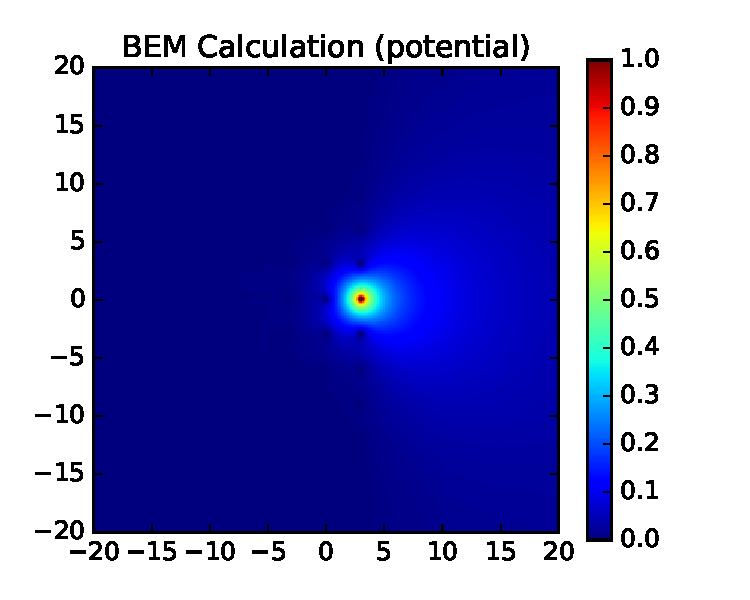
\includegraphics[height=0.65\textheight]{parallel-near-d11.pdf}

        \scriptsize 3D BEM, parallel wires, sliced at Y=0.
      \end{center}
    \end{column}
  \end{columns}

  \begin{center}
    Initial, qualitative agreement.  More checks needed.
  \end{center}

\end{frame}

\begin{frame}{Weighting Potential - 2D vs. 3D wire pattern}

  \vspace{-5mm}

  \begin{columns}
    \begin{column}{0.5\textwidth}
      \begin{center}
        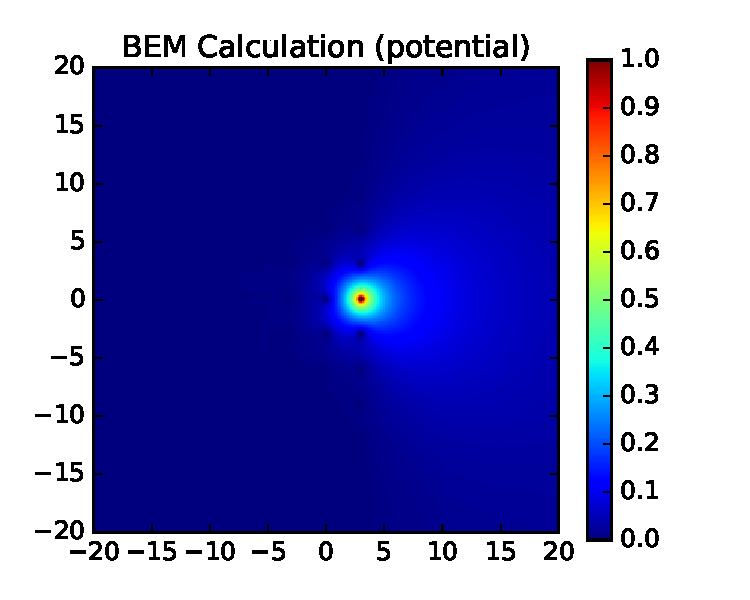
\includegraphics[height=0.65\textheight]{parallel-near-d11.pdf}

        \scriptsize Parallel wires
      \end{center}
    \end{column}
    \begin{column}{0.5\textwidth}
      \begin{center}
        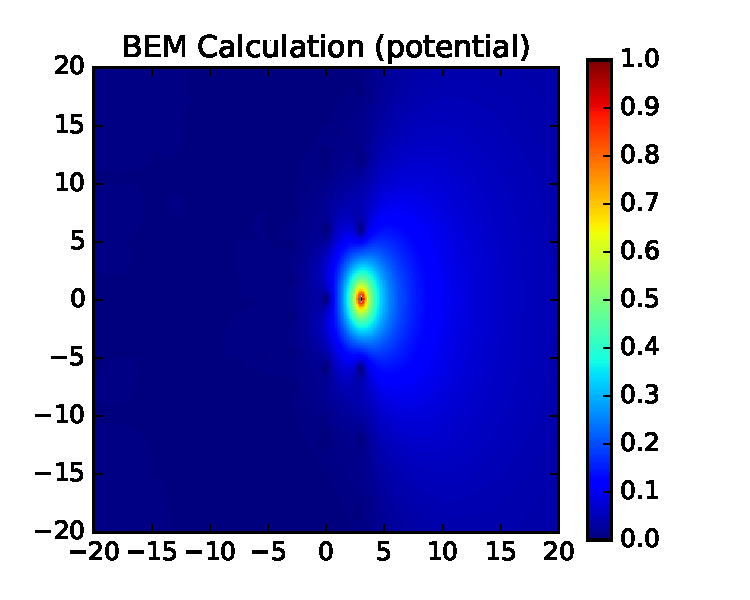
\includegraphics[height=0.65\textheight]{uboone-near-d11.pdf}

        \scriptsize \microboone wires.
      \end{center}
    \end{column}
  \end{columns}

  \begin{center}
    Clear distortion in extent and shape.  Not surprising.
  \end{center}

\end{frame}


\begin{frame}
  \frametitle{An Initial E-Field Calculation}
  \begin{center}
    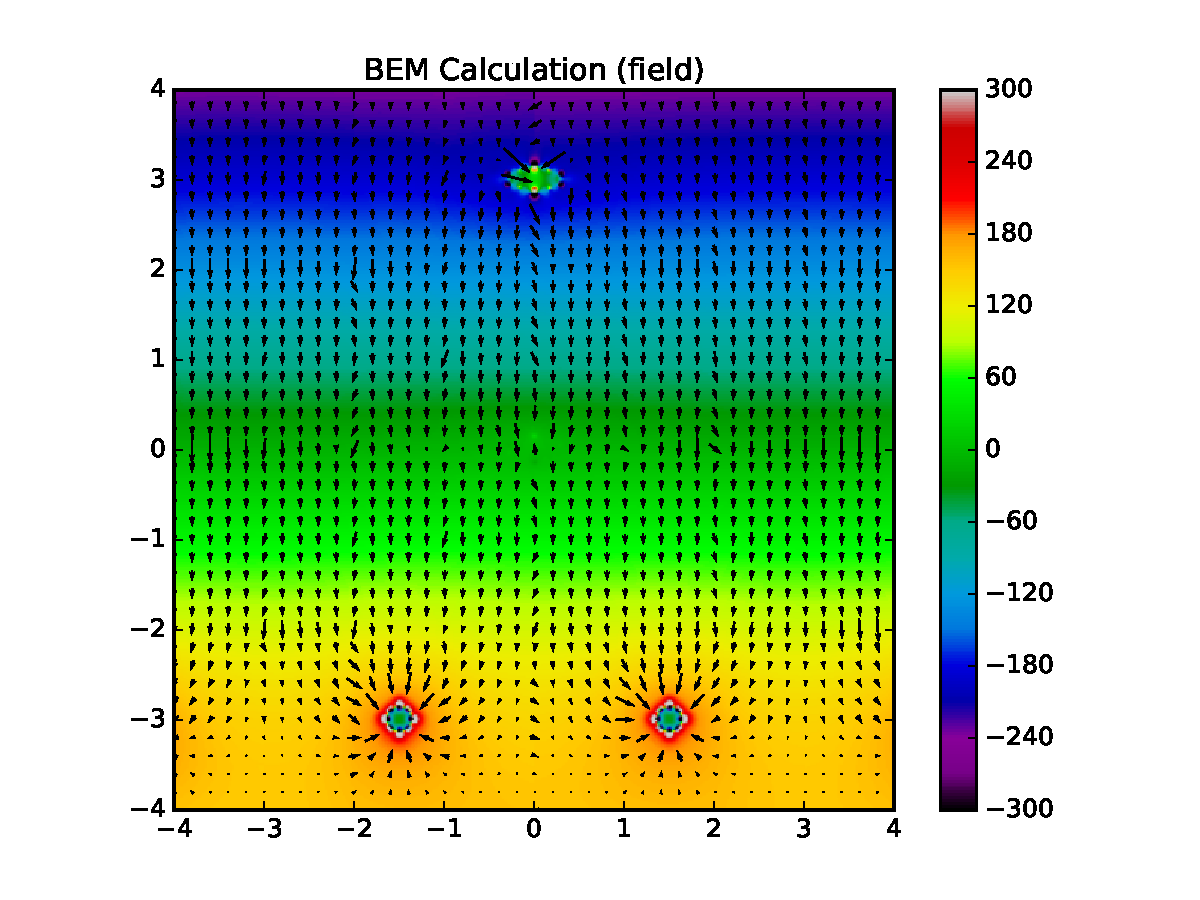
\includegraphics[height=0.7\textheight]{uboone-drift-field-pot-tight.pdf}
  \end{center}
  \vspace{-5mm}
  
  \begin{itemize}\footnotesize
  \item Square wires?  Large fluctuations near wires?
  \item Weird discontinuities/artifacts in the volume?  
  \end{itemize}
  \onslide<2>{
  \begin{center}
    \LARGE What's going on?!~~~~~~$\longrightarrow$
  \end{center}}
\end{frame}

\begin{frame}
  \frametitle{What are These Problems?}
  Ultimately they are all due to \textbf{mesh granularity}.  
  \vspace{5mm}
  \begin{itemize}
  \item Near-surface problems:
    \begin{itemize}\footnotesize
    \item Mesh approximates real shape with triangles 
      \begin{itemize}\scriptsize
      \item[$\Rightarrow$] circular cross-section wires $\to$ square/hexagon
      \end{itemize}
    \item Mesh has sharp edges and points 
      \begin{itemize}\scriptsize
      \item[$\Rightarrow$] large local fields (as it should be!)
      \end{itemize}
    \end{itemize}
  \item In-volume problems:
    \begin{itemize}\footnotesize
    \item BEM evaluates a sum over pairs of mesh triangles.
    \item Triangles are sub-sampled, more for nearby pairs, less for far.
    \item As one goes from ``close'', ``medium'' and ``far'' pairs, different number of sub-samples used.
    \item[$\Rightarrow$] visible artifacts at borders of these different volume domains.
    \end{itemize}
  \end{itemize}
  \vspace{5mm}
  There are ``knobs'' that \textbf{can and must be tuned} to control this.
  
  All trade off running time for accuracy.
\end{frame}

\begin{frame}
  \frametitle{Intial Stepping Tests}
  \begin{center}
    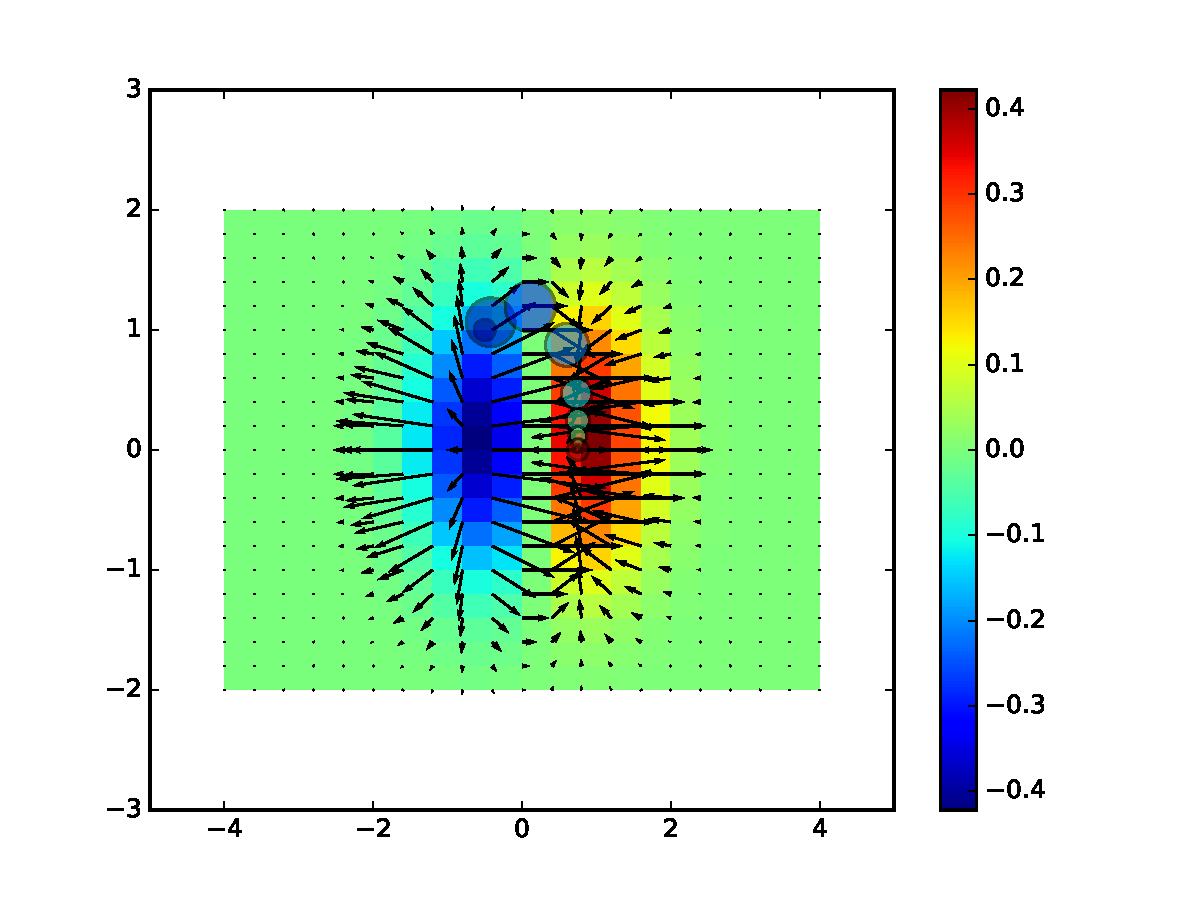
\includegraphics[width=0.8\textwidth,clip,trim=0 10mm 0 10mm]{initial_stepping_test2.pdf}    
  \end{center}

  \scriptsize
  Just a made-up test ``velocity potential''.  Arrows show local
  velocity.  Circles are steps with time as color and step distance as
  area.

\end{frame}


\begin{frame}
  \frametitle{The Software - Main Dependencies}

  \href{http://www.bempp.org/}{BEM++}
  \begin{itemize}
  \item Solves Laplace, Helmholtz and Maxwell eqns using BEM
  \item C++ with Python interface.
  \item General, but low-level.  Requires some understanding.
  \item Multithreaded.
  \end{itemize}

  \href{http://gmsh.info}{GMSH}
  \begin{itemize}
  \item 3D Grid generator and visualization.
  \item Supports bot volume and surface meshes.
  \item Interactive and scripted geometry definition.
  \end{itemize}

  Python:
  \begin{itemize}
  \item NumPy, Matplotlib, MayaVi, Sqlalchemy/Sqlite3, Click
  \item all wrapped together by \textbf{LARF} $\rightarrow$
  \end{itemize}
\end{frame}

\begin{frame}[fragile]
  \frametitle{LARF - \textbf{L}iquid \textbf{Ar}gon TPC \textbf{F}ield Calculator}

  Some features:
  \begin{itemize}
  \item Standard Python installation.
  \item Command line and Python module interface.
  \item Simple config file specifies the many input parameters.
  \item Handles everything from geometry to solving to stepping.
  \item Results stored in Sqlite3 database file.
  \item Multiple data export methods (Numpy \texttt{.npz}, VTK)
  \item Built-in visualization (2D/matplotlib, 3D/mayavi).
  \end{itemize}

  Code and docs on GitHub:
  \begin{center}
    \url{https://github.com/brettviren/larf}.    
  \end{center}
\end{frame}

\begin{frame}

  LARF status:

  \begin{itemize}\footnotesize
  \item About \textbf{90\% feature complete}
    \begin{itemize}\scriptsize
    \item (the remaining 90\% will still take a lot of work!)
    \item ``done'': geometry, meshing, ES potential, R-S potential,
      mobility/velocity, volume rastering, drift stepping, and current
      sampling.
    \end{itemize}
  \item Lots of documentation and some unit tests.
  \item[$\rightarrow$] Brave users could give it a try.    
  \end{itemize}

  To do:

  \begin{itemize}\footnotesize
  \item Lots of intermediate diagnostic plots to add.
  \item Systematic end-to-end validation:
    \begin{itemize}\scriptsize
    \item Various ``does it look right'' visualizations.
    \item Comparison to 2D Garfield and with Leon's 3D FEM.
    \end{itemize}
  \item Study response \textit{vs.} step starting positions.
  \item[$\rightarrow$] Apply to MicroBooNE data to see if removes known problems!
  \item Tune precision knobs.  If required, consider hybrid BEM/FEM.
    \begin{itemize}\scriptsize
    \item BEM++ hooks into \href{https://fenicsproject.org/}{FEniCS} FEM.
    \end{itemize}
  \end{itemize}
\end{frame}

\end{document}